\clearpage
\section{Control Flow Concepts} % (fold)
\label{sec:control_flow_concepts}

Programming is about designing code that commands the computer to perform actions. Earlier chapters have introduced the \nameref{sub:program}, \nameref{sub:procedure}, and \nameref{sub:function} artefacts into which you can enter these instructions, but have not elaborated on the actions that you can perform.

Most of a program's actual work will be carried out in \nameref{sub:assignment_statement}s, and through \nameref{sub:procedure call}s and \nameref{sub:function_call}s. These are the main commands, allowing you to alter values stored in memory and to execute stored instructions. The remaining commands relate to controlling the order in which the computer performs the instructions; called \textbf{control flow statements}.

This chapter introduces the following kinds of instructions. You can use these to get the computer to perform certain \textbf{actions} within your program.
\begin{itemize}
  \item \nameref{sub:if_statement}: Run some code if a condition is true.
  \item \nameref{sub:case_statement}: Selectively run a branch of code.
  \item \nameref{sub:compound_statement}: Group statements together.
  \item \nameref{sub:pre_test_loop}: Loop after testing a condition.
  \item \nameref{sub:post_test_loop}: Loop then test a condition.
\end{itemize}

In addition to these actions, you will need have a look at an existing \textbf{artefact}:
\begin{itemize}
  \item \nameref{sub:boolean_data}: An existing \nameref{sub:type} that has either a \emph{true} or \emph{false} value.
\end{itemize}

\bigskip

You may need to revise the following programming artefacts:
\begin{itemize}
  \item \nameref{sub:program}: The idea of building your own programs.
  \item \nameref{sub:procedure}: Creating your own Procedure, as well as calling Procedures from libraries.
  \item \nameref{sub:function}: Creating your own Functions, as well as calling Functions from libraries.
\end{itemize}

The following programming terminology will also be used in this Chapter:
\begin{itemize}
  \item \nameref{sub:statement}: An instruction performed in your code.
  \item \nameref{sub:type}: A kind of data used in your code.
\end{itemize}

The example for this chapter is a guessing game, where the user is guessing a number between 1 and 100. An example of this program executing is shown in Figure \ref{fig:control-flow-guess-num}.

\begin{figure}[h]
   \centering
   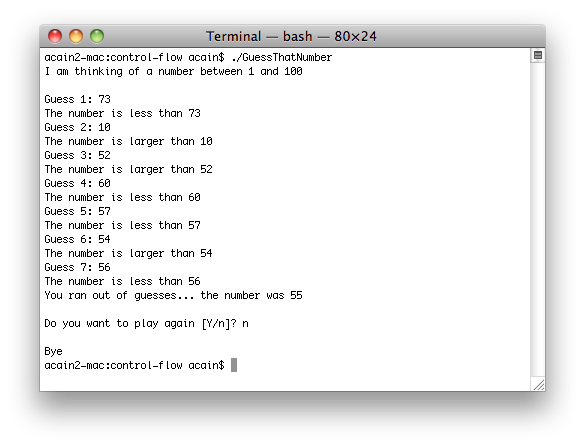
\includegraphics[width=0.5\textwidth]{./topics/control-flow/images/GuessThatNumber} 
   \caption[Guess That Number Terminal]{Guess that Number run from the Terminal}
   \label{fig:control-flow-guess-num}
\end{figure}

\clearpage
\subsection{Boolean Data} % (fold)
\label{sub:boolean_data}

The Boolean\footnote{Named after George Bool's Boolean logic.} Data Type is a \nameref{sub:type} used to represent \textbf{truth}. A Boolean value will either be \textbf{true} or \textbf{false}. These values are used extensively in the control flow statements to determine the action to perform.

\begin{figure}[h]
   \centering
   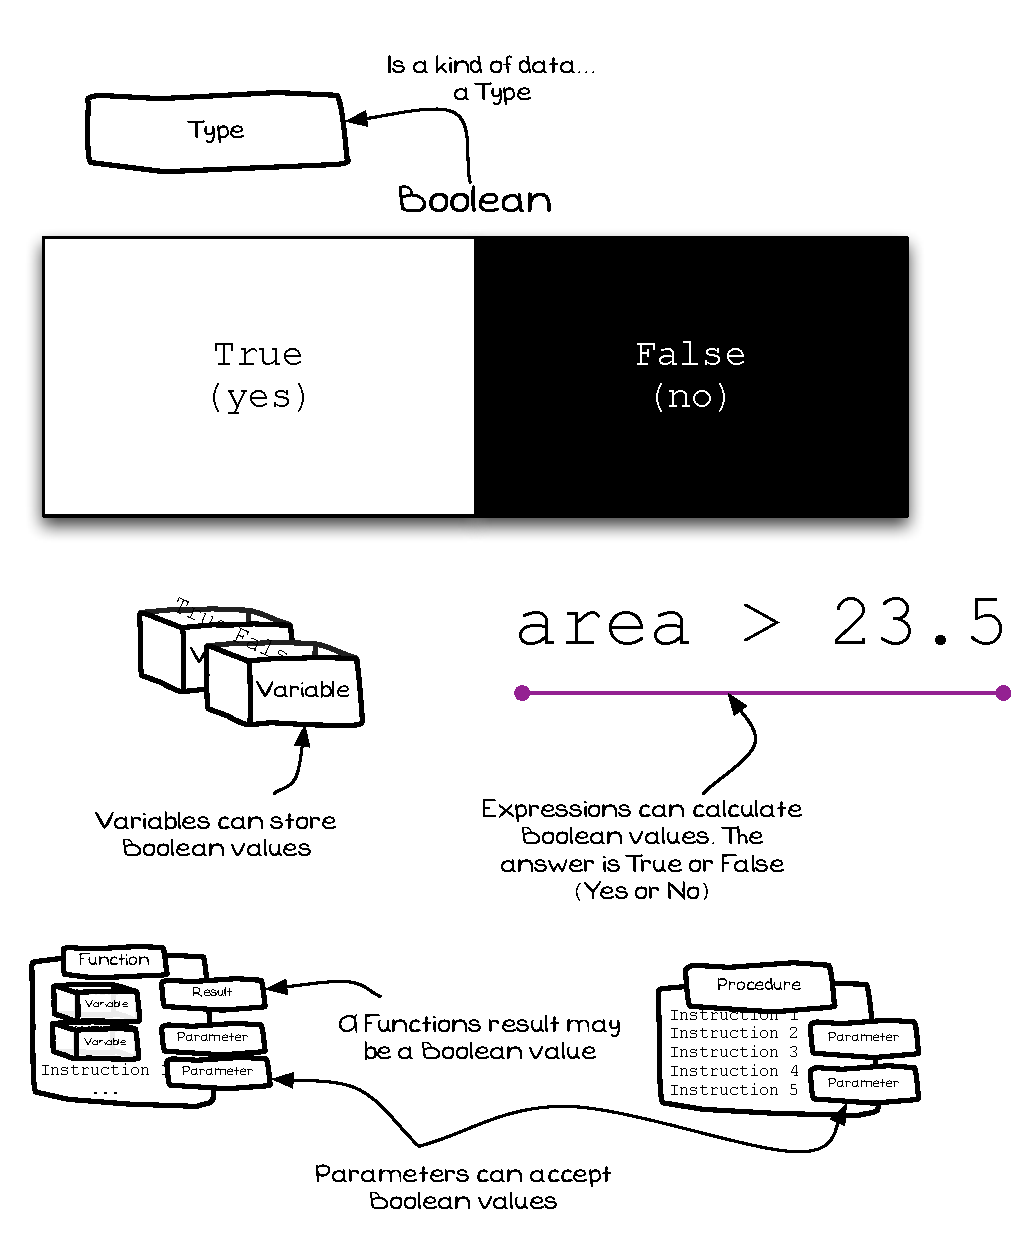
\includegraphics[width=0.8\textwidth]{./topics/control-flow/diagrams/BooleanData} 
   \caption{Boolean data represents truth}
   \label{fig:boolean-data}
\end{figure}

\mynote{
\begin{itemize}
  \item Boolean is an existing \textbf{artefact}, it is a \nameref{sub:type} that has been defined to represent truth values.
  \item A Boolean value is either \textbf{true} or \textbf{false}. You can also think of these as \emph{yes} and \emph{no}.
  \item Boolean values are used in most of the control flow statements.
  \item The Boolean type can be used in the same way as other types.
\end{itemize}
}
% subsection boolean_data (end)

\clearpage
\subsubsection{Comparisons} % (fold)
\label{sub:comparisons}

Comparisons are a common way of getting Boolean values in your code. These \nameref{sub:expression}s allow you to compare two values to check for a given condition. For example, the Expression shown in Figure \ref{fig:boolean-data} is asking if the \emph{value} in the \texttt{area} variable is larger than \texttt{23.5}. The result of this expression will be either \texttt{true} or \texttt{false} depending on the current value stored in \texttt{area}. Table \ref{tbl:bool-expr-sample} lists some example values for this expression, given different values stored in the \texttt{area} variable.

\begin{table}[h]
  \centering
  \begin{tabular}{|c|c|}
    \hline
    \textbf{Value in \texttt{area}} & \textbf{\texttt{area > 23.5}} \\
    \hline
    \texttt{73.2} & \texttt{true} \\
    \hline
    \texttt{-2.5} & \texttt{false} \\
    \hline
    \texttt{23.5} & \texttt{false} \\
    \hline
  \end{tabular}
  \caption{Example values for the expression \texttt{area > 23.5}}
  \label{tbl:bool-expr-sample}
\end{table}

Programming languages offer a range of different comparison operators. These typically include comparisons to check if values are the same or different, and to check if one value is larger or small than another. The different operators for C and Pascal are listed in Table \ref{tbl:comparisons}.

\begin{table}[h]
  \centering
  \begin{tabular}{|c|c|c|c|}
    \hline
     & \textbf{Description} & \textbf{C} & \textbf{Pascal} \\
    \hline
    \textbf{Equal} & Are the values the same? & \texttt{a == b} & \texttt{a = b} \\
    \hline
    \textbf{Not Equal} & Are the values different? & \texttt{a != b} & \texttt{a <> b} \\
    \hline
    \textbf{Larger Than} & Is the left value larger than the right? & \multicolumn{2}{c|}{\texttt{a > b}}  \\
    \hline
    \textbf{Less Than} & Is the left value smaller than the right? & \multicolumn{2}{c|}{\texttt{a < b}}  \\
    \hline
    \textbf{Larger Or Equal} & Is the left value equal or larger than the right? & \multicolumn{2}{c|}{\texttt{a >= b}}  \\
    \hline
    \textbf{Less Or Equal} & Is the left value smaller or equal to the right? & \multicolumn{2}{c|}{\texttt{a <= b}}  \\
    \hline
    
  \end{tabular}
  \caption{Comparison Operators}
  \label{tbl:comparisons}
\end{table}

\mynote{
\begin{itemize}
  \item Comparisons can only be performed between \textbf{two} values.
  \item The values on either side of the comparison are \nameref{sub:expression}s, allowing you to calculate the values being compared.
\end{itemize}
}

\csection{
C uses a double equal (\texttt{==}) for comparison as the single equals (\texttt{=}) is used for assignment.
}

% subsection comparisons (end)

\clearpage
\subsubsection{Logical Operators} % (fold)
\label{sub:logical_operators}

The comparison operators allow you to compare \emph{two} values. This is very useful, but in itself is incomplete. What, for example, do you do when you want to compare three or more values? While you are limited to two values with the comparison operators, there are other operators that allow you to \textbf{combine} Boolean expressions. This will enable you to combine together multiple Boolean values into a single Expression.

There are four main \emph{logical operators}: \textbf{and}, \textbf{or}, \textbf{xor}, and \textbf{not}. Each of these operators works on two Boolean values, combining them to give a new Boolean value. For example, the \emph{and} operator allows you to check if \emph{both} of the expressions are true. The expression \texttt{area > 0 and area < 10} will be true only when area is both larger than zero and less then ten.

\begin{figure}[h]
   \centering
   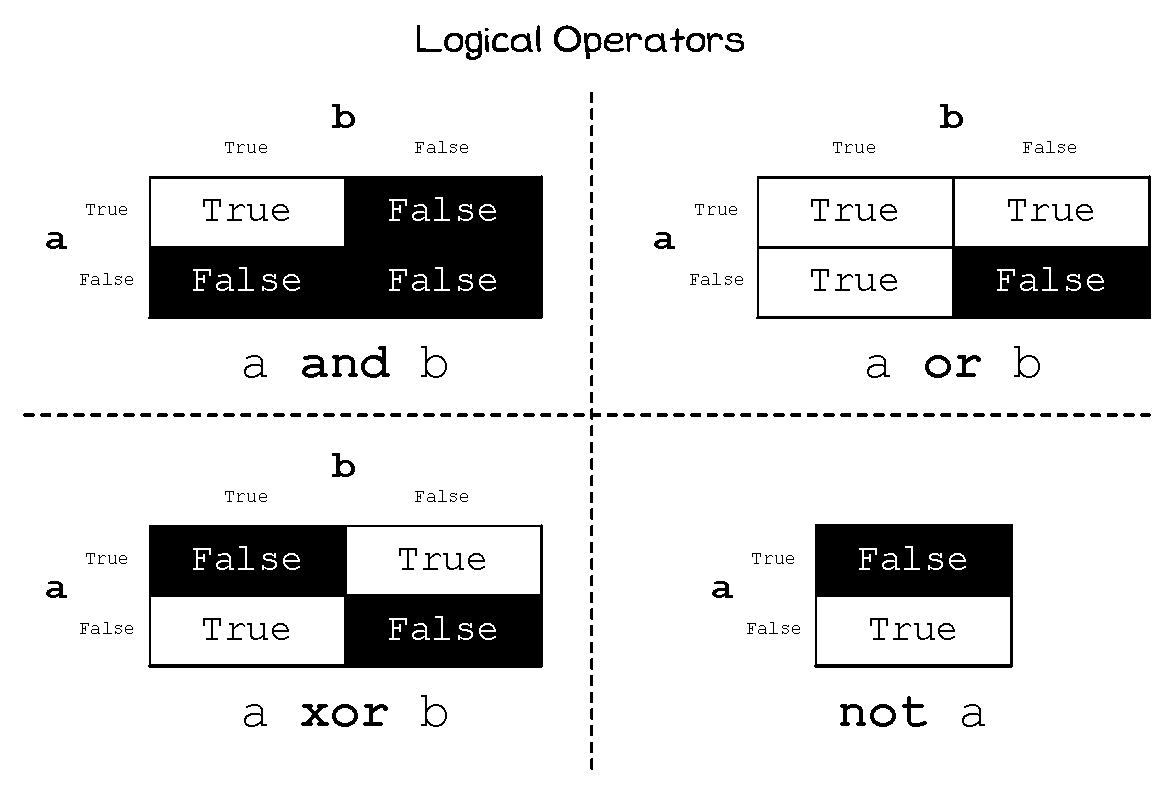
\includegraphics[width=0.7\textwidth]{./topics/control-flow/diagrams/LogicalOperators} 
   \caption{Logical Operators combine Boolean values}
   \label{fig:logical-operators}
\end{figure}

\begin{table}[h]
  \centering
  \begin{tabular}{|c|c|c|c|}
    \hline
     & \textbf{Description} & \textbf{C} & \textbf{Pascal} \\
    \hline
    \textbf{And} & Are both values True? & \texttt{a \&\& b} & \texttt{a and b} \\
    \hline
    \textbf{Or} & Is at least one value True? & \texttt{a || b} & \texttt{a or b} \\
    \hline
    \textbf{Xor} & Is one value True, and the other False? & \texttt{a \^{} b} & \texttt{a xor b} \\
    \hline
    \textbf{Not} & Is the value False? & \texttt{!a} & \texttt{not a}  \\
    \hline
  \end{tabular}
  \caption{Logical Operators}
  \label{tbl:logical-operators}
\end{table}

\begin{table}[h]
  \centering
  \begin{tabular}{|c|c|c|c|c|c|}
    \hline
    \multirow{2}{*}{area }& \multirow{2}{*}{\texttt{area > 0}} & \multirow{2}{*}{\texttt{area < 10}} & \multicolumn{3}{c|}{\texttt{area > 0 {\textbf{\ldots}} area < 10}} \\
    \cline{4-6}
     &  &  & \textbf{and} & \textbf{or} & \textbf{xor} \\
    \hline
    \texttt{\textbf{5}} & True & True & True & True & False \\
    \hline
    \texttt{\textbf{27}} & True & False & False & True & True \\
    \hline
    \texttt{\textbf{0}} & False & True & False & True & True \\
    \hline
  \end{tabular}
  \caption{Example Logical Expressions}
  \label{tbl:example_logical_expr}
\end{table}

\mynote{
\begin{itemize}
  \item Table \ref{tbl:example_logical_expr} has some example expressions.
  \item The tables in Figure \ref{fig:logical-operators} show the values of the different logical operators. These are known as \textbf{Truth Tables}.
  \item Table \ref{tbl:logical-operators} outlines the different logical operators, and how they are coded in C and Pascal.
\end{itemize}
}



% subsection boolean_logic (end)

\subsection{Branching} % (fold)
\label{sub:branching}

There are two main ways of controlling the sequence of actions in a program. The first of these is called \textbf{branching}, or \textbf{selection}. Branching allows you to get the computer to take one of a number of paths based on the value of a \emph{condition}.

\begin{figure}[h]
   \centering
   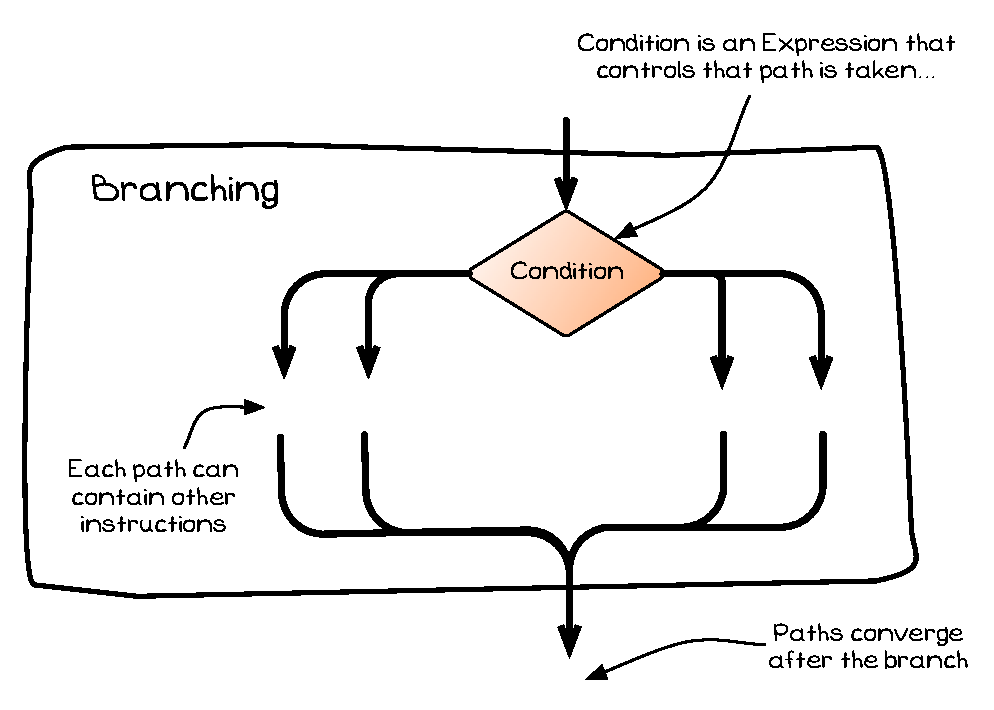
\includegraphics[width=0.8\textwidth]{./topics/control-flow/diagrams/Branching} 
   \caption{Branching commands the computer to take one of a number of possible paths}
   \label{fig:branching}
\end{figure}

\mynote{
\begin{itemize}
  \item Branching is a kind of \textbf{action}. You can command the computer to take of a number of paths.
  \item A branch has a \textbf{condition} that is evaluated, and based on the condition the computer takes one path.
  \item The branch is the act of choosing the path, when its command is performed the computer evaluates the condition and then moves to the instructions in the indicated path.
  \item Languages usually offer two kinds of branching statements:
  \begin{itemize}
    \item \nameref{sub:if_statement} to select between two paths based on a Boolean expression.
    \item \nameref{sub:case_statement}  to select a path based on an ordinal\footnote{Integers and Characters are ordinal values. Ordinal values have a defined sequence, so it is possible to say which value comes next in the sequence. Integers are Ordinal as you can say that the number after 1 is 2. Real numbers are not ordinal as you cannot say which value comes next in the sequence.} value.
  \end{itemize}
  \item The Branch will have one entry point, and one exit point. This feature allows you to combine statements together like building blocks. This idea comes from the principles of \textbf{Structured Programming}, where each component in the code should have a single entry and exit point.
\end{itemize}
}


% subsection branching (end)
\clearpage
\subsubsection{If Statement} % (fold)
\label{sub:if_statement}

The if statement is the most frequently used branching statement. It allows you to selectively run code based on the value of a Boolean expression (the condition). The if statement has an optional \emph{else} branch that is executed when the condition is false.

\begin{figure}[h]
   \centering
   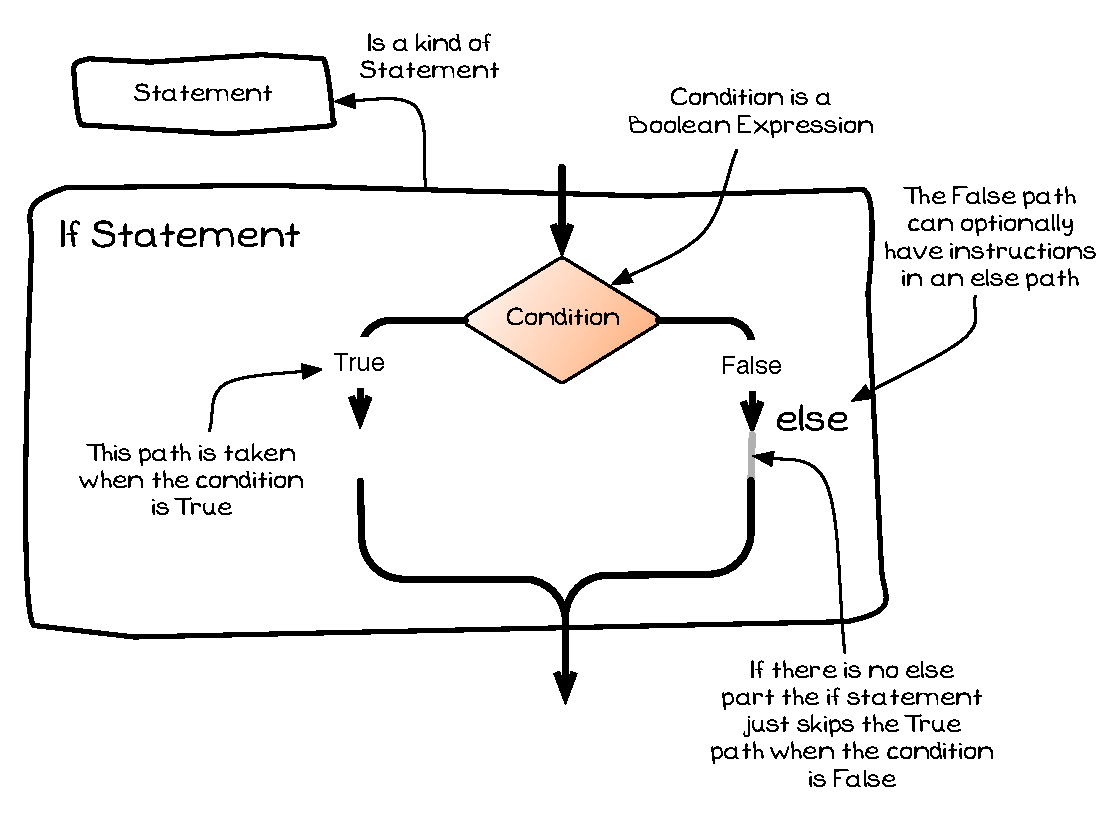
\includegraphics[width=\textwidth]{./topics/control-flow/diagrams/IfStatement} 
   \caption{If statement lets you selectively run a branch of code}
   \label{fig:branching-if-statement}
\end{figure}

\mynote{
\begin{itemize}
  \item An if statement is an \textbf{action}. It allows you to command the computer to select a path based on a Boolean expression.
  \item The if statement has two branches, one that is taken when the condition is True, the other when it is False.
  \item The False branch may \emph{optionally} have instructions that are carried out when the condition is False. 
  \item If there are no instructions you want performed when the condition is False you do not need to include an else branch, and the if statement will just skip the True branch when the condition is False.
  \item The if statement has one entry point, two paths, and then one exit point.
\end{itemize}
}


% subsection if_statement (end)
\clearpage
\subsubsection{Case Statement} % (fold)
\label{sub:case_statement}

The case statement is the second kind of branching statement. This allows you to create paths that execute based on matching a value from an expression. This allows one case statement to handle many alternative paths.

\begin{figure}[h]
   \centering
   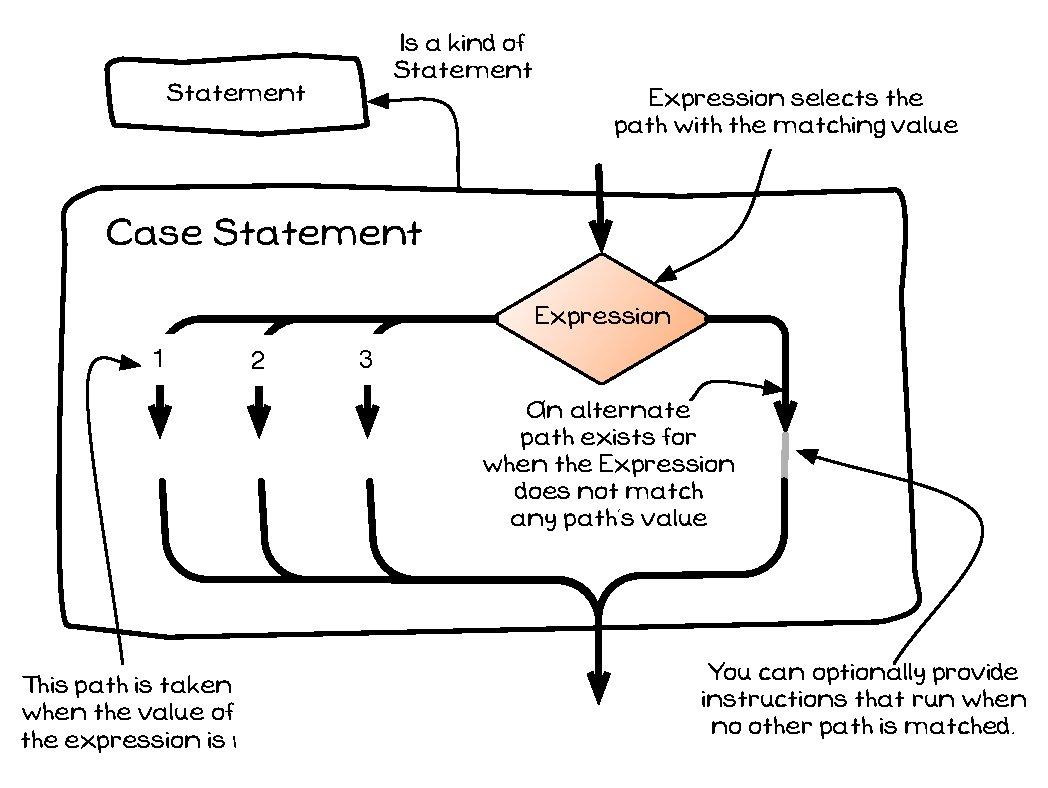
\includegraphics[width=\textwidth]{./topics/control-flow/diagrams/CaseStatement} 
   \caption{Case statement selectively runs multiple branches of code}
   \label{fig:branching-case-statement}
\end{figure}

\mynote{
\begin{itemize}
  \item The case statement is a kind of \textbf{action}. It allows you to command the computer to select a path based upon the value of an expression.
  \item Each path within the Case Statement has a value. When the computer executes the case statement the path values are used to determine which path will be taken.
  \item In C and Pascal the Case Statement only works with Ordinal Values. This limits you to using Character or Integer values within the Case Statement's Expression.
  \item The Case Statement has one entry point, multiple paths, and then one exit point.
\end{itemize}
}

% section case_statement (end)

\clearpage
\subsection{Looping} % (fold)
\label{sub:looping}

There are two main ways of controlling the sequence of actions in a program. The first was \textbf{branching}, the second is called \textbf{looping}, or \textbf{repetition}. The language's looping statements allow you to have actions repeated.

\begin{figure}[h]
   \centering
   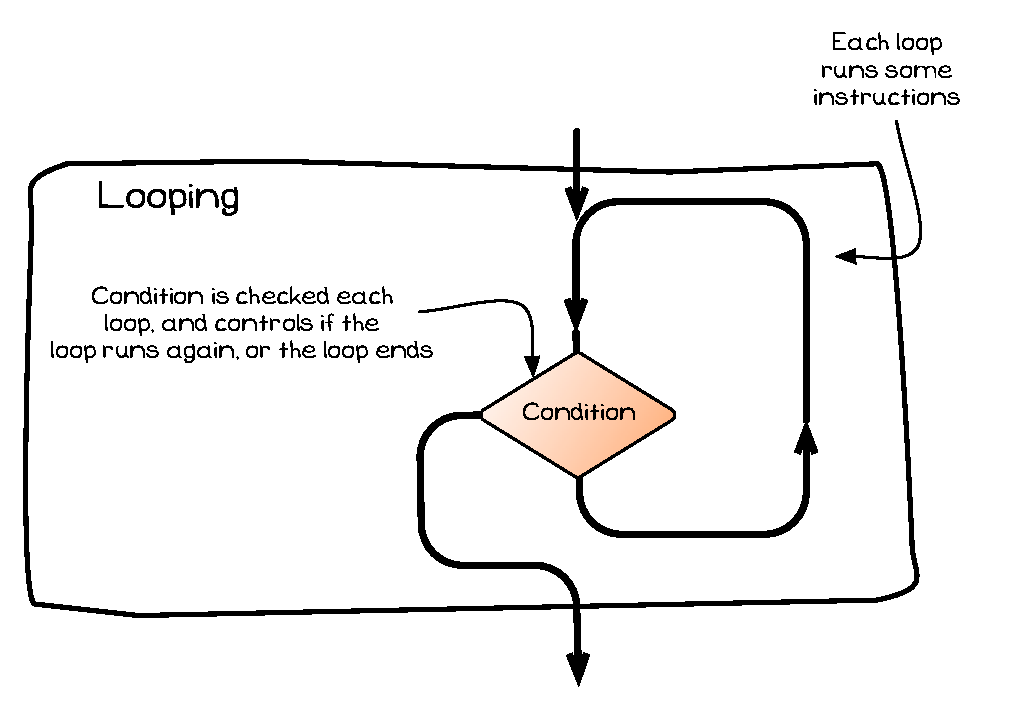
\includegraphics[width=0.9\textwidth]{./topics/control-flow/diagrams/Looping} 
   \caption{Looping commands the computer to repeat a path}
   \label{fig:looping}
\end{figure}

\mynote{
\begin{itemize}
  \item Looping is a kind of \textbf{action}. You can command the computer to repeat the steps within a path.
  \item A number of steps are performed each loop:
  \begin{itemize}
    \item The instructions within the loop are executed.
    \item The \emph{condition} is checked, and the instructions are either run again or the loop ends.
  \end{itemize}
  \item The \emph{condition} may be checked before or after the instructions are executed, giving two kinds of loops:
  \begin{itemize}
    \item \nameref{sub:pre_test_loop}: Repeats instructions 0 or more times.
    \item \nameref{sub:post_test_loop}: Repeats instructions 1 or more times.
  \end{itemize}
  \item As with Branching, the Looping Statements have a single entry and a single exit in keeping with the principles of \textbf{Structured Programming}.
\end{itemize}
}


% subsection looping (end)
\clearpage
\subsubsection{Pre-Test Loop} % (fold)
\label{sub:pre_test_loop}

The Pre-Test Loop is a looping statement that allows code to be run 0 or times. The loop checks the condition at the start, and if the condition is True the loop's body is executed. At the end of the loops body the computer jumps back to the condition, checking it again to determine if the loop's body should execute again. If the condition is False when it is checked the loop jumps ends, and control jumps to the next statement in the code.

\begin{figure}[h]
   \centering
   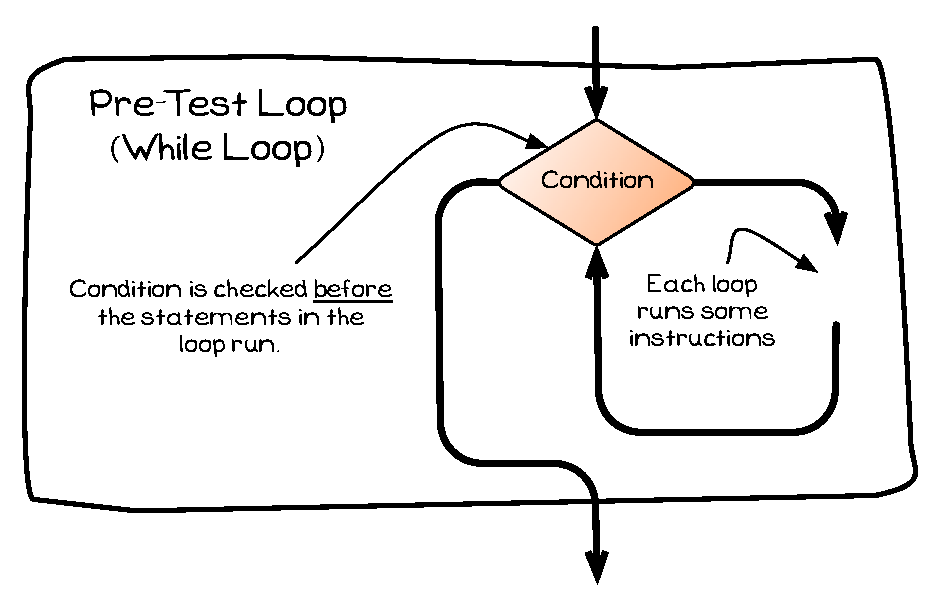
\includegraphics[width=\textwidth]{./topics/control-flow/diagrams/PreTestLoop} 
   \caption{The Pre-Test Loop checks the condition, then runs the loop's body}
   \label{fig:looping-pre-test}
\end{figure}

\mynote{
\begin{itemize}
  \item A pre-test loop is an \textbf{action}, creating a loop in the code's sequence of instructions.
  \item The standard pre-test loop is the \textbf{while statement}.
  \item A pre-test loop allows instructions to be run 0 or more times.
  \item The condition is checked when the loop's code is entered, and it is checked again at the end of each loop.
\end{itemize}
}


% subsection post_test_loop (end)
\clearpage
\subsubsection{Post-Test Loop} % (fold)
\label{sub:post_test_loop}

The Post-Test Loop is a looping statement that allows code to be run 1 or times. The post-test loop places the condition after the body of the loop. This means that the first time through the body of the loop must execute before the condition is checked. When it gets to the end of the body, the loop's condition is checked and the computer either jumps back to the start of the loop to repeat the body, or the loop ends and control flows on to the next statement in the code.

There are two common variants for the post-test loop: \texttt{\textbf{do...while}} and \texttt{\textbf{repeat...until}}. These work in the same way, in that they test the condition after the loop body, but the conditions they use will be different. The \textbf{\texttt{do...while}} loop repeats the body of the loop when its condition is \textbf{true}, \textbf{\texttt{repeat...until}} repeats the body of the loop when its condition is \textbf{false}. When implementing a post-test loop you must make sure that the condition you use matches the kind of loop supported by your language.

\begin{figure}[h]
   \centering
   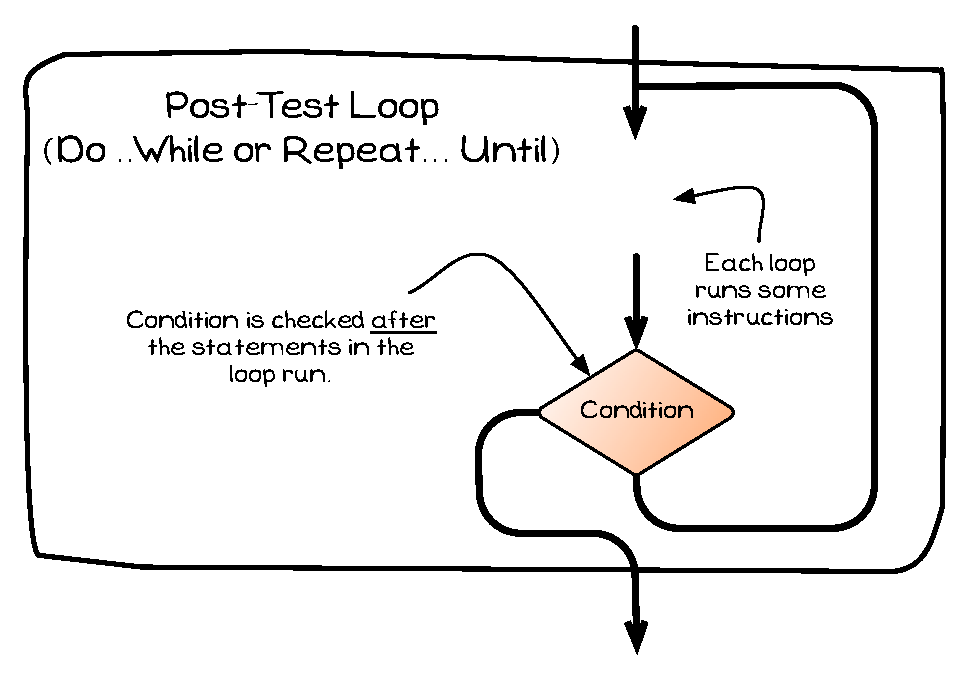
\includegraphics[width=0.9\textwidth]{./topics/control-flow/diagrams/PostTestLoop} 
   \caption{The Post-Test Loop runs the loops body, then checks the condition}
   \label{fig:looping-post-test}
\end{figure}

\mynote{
\begin{itemize}
  \item A post-test loop is an \textbf{action}, creating a loop in the code's sequence of instructions.
  \item A post-test loop allows instructions to be run 1 or more times.
  \item The condition is checked after the loop's body is executed, with control jumping back to the start if needed.
\end{itemize}
}

\csection{C includes support for the \textbf{\texttt{do...while}} loop.}
\passection{Pascal includes support for the \textbf{\texttt{repeat...until}} loop.}

% subsection post_test_loop (end)

\clearpage
\subsection{Jumping} % (fold)
\label{sub:jump}

The jump statements allow you to alter the sequence of instructions in the code, getting the computer to jump to another instruction.

\begin{figure}[h]
   \centering
   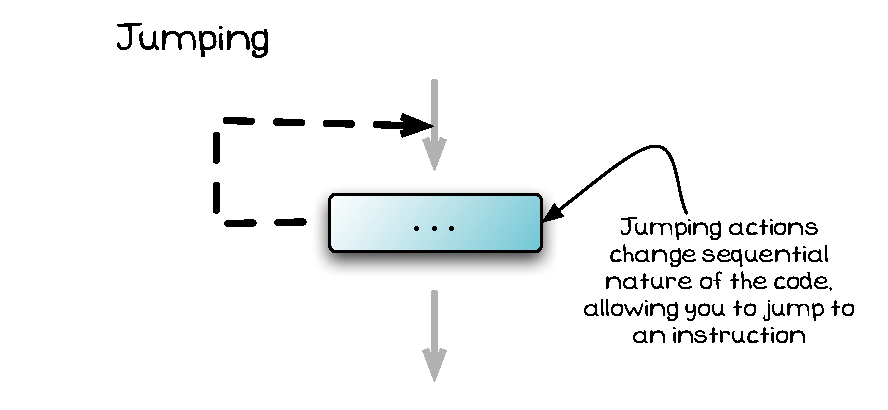
\includegraphics[width=\textwidth]{./topics/control-flow/diagrams/JumpStatements} 
   \caption{Jump Statements cause control to jump to another location in the code}
   \label{fig:looping-jump-statements}
\end{figure}

\mynote{
\begin{itemize}
  \item The jump statements are \textbf{actions}, they allow you to alter the standard sequence of the instructions and have the computer jump to a another location in the instructions.
  \item \textbf{Structured Programming} was proposed as a means of providing order and structure to the control flow through the code. These jump statements complicate this sequential flow, but in some cases they are able to simplify code.
  \item Structured jump statements allow you to control the sequence of actions related to a \nameref{sub:looping} statement, a \nameref{sub:function}, or a \nameref{sub:procedure}. These work the looping and procedural structures used in structured programming.
  \item Unstructured jump statements allow you to jump to any instruction within the code. You need to be aware that these statements exist, but they should not be used.
\end{itemize}
}

% subsection jump_statements (end)
\clearpage
\subsubsection{Break} % (fold)
\label{sub:break}

The break statement is used to jump out of the current loop, in effect terminating the loop early. This is useful for ending the current loop, skipping all future cycles.

\begin{figure}[h]
   \centering
   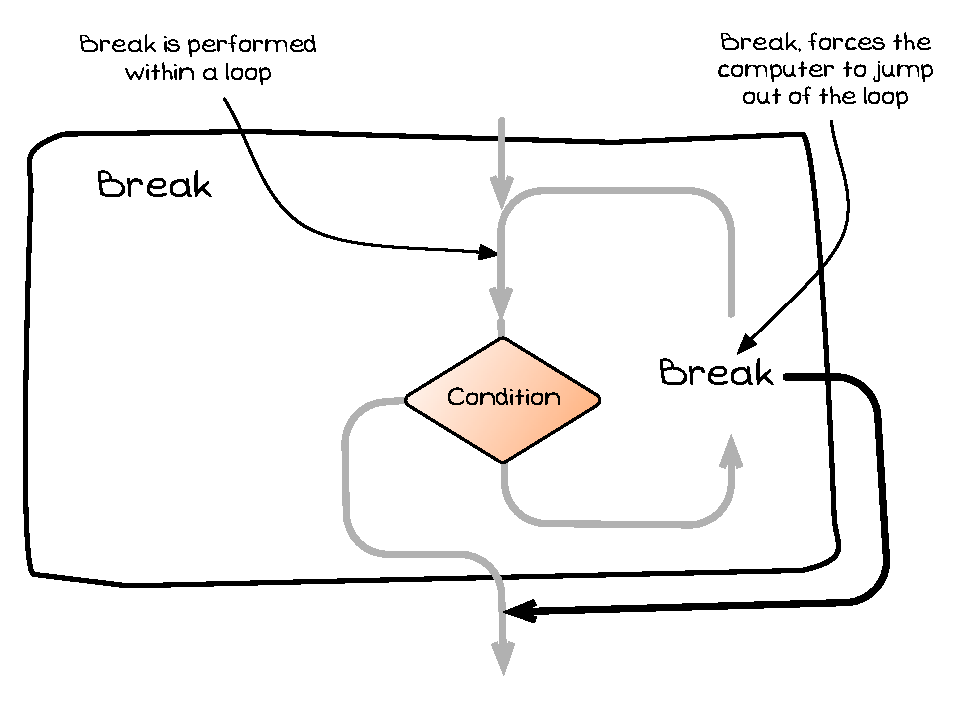
\includegraphics[width=\textwidth]{./topics/control-flow/diagrams/Break} 
   \caption{The Break Statement allows you to end a loop early}
   \label{fig:break}
\end{figure}

\mynote{
\begin{itemize}
  \item The break statement is an \textbf{action}, allowing you to jump to the end of the current loop.
  \item The break statement should be coded within an \nameref{sub:branching} statement that checks if the loop should terminate early.
\end{itemize}
}


% subsection break (end)
\clearpage
\subsubsection{Continue} % (fold)
\label{sub:continue}

The continue statement is used to jump to the condition of the current loop. This is useful for skipping the processing of the current loop, but to allow the loop to continue for the next cycle.

\begin{figure}[h]
   \centering
   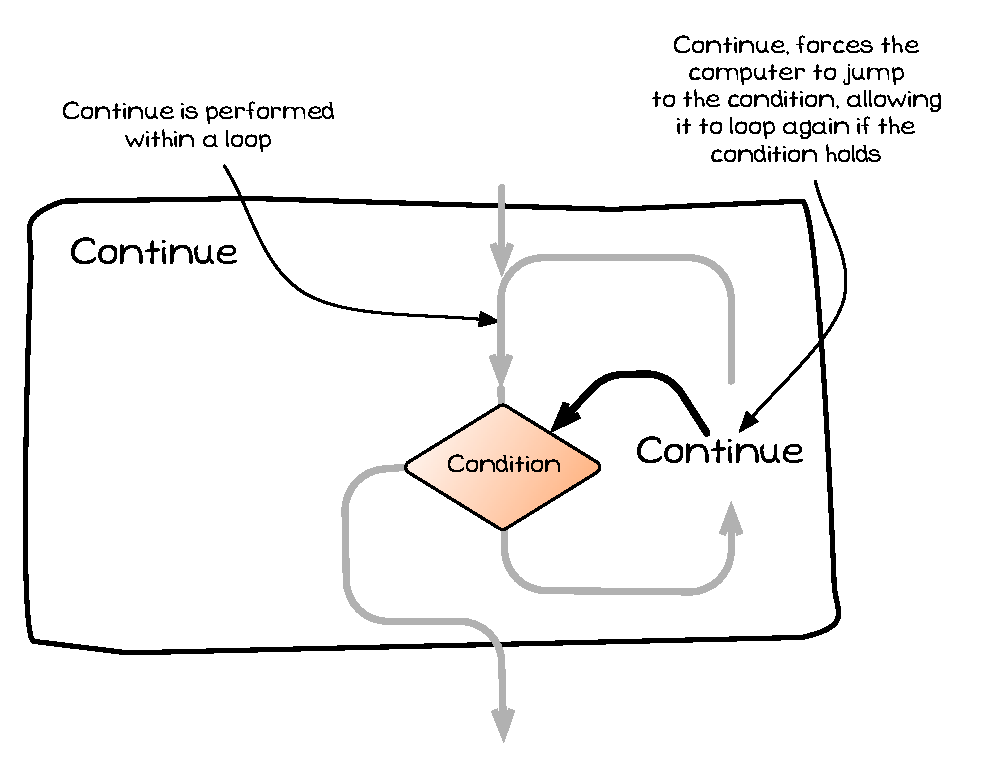
\includegraphics[width=\textwidth]{./topics/control-flow/diagrams/Continue} 
   \caption{The continue Statement allows you to jump to the condition, skipping the remainder of the code in the loop but allowing the loop to continue}
   \label{fig:continue}
\end{figure}

\mynote{
\begin{itemize}
  \item The continue statement is an \textbf{action}, allowing you to jump to the condition of the current loop.
  \item The continue statement should be coded within an \nameref{sub:branching} statement that checks if the loop should skip processing of the current cycle.
\end{itemize}
}


% subsection break (end)
\clearpage
\subsubsection{Exit} % (fold)
\label{sub:exit}

The exit statement, or the return in C, ends the current \nameref{sub:function} or \nameref{sub:procedure}. This is useful for skipping the rest of the processing of the Function or Procedure, exiting it early and returning to the calling code. 

\begin{figure}[h]
   \centering
   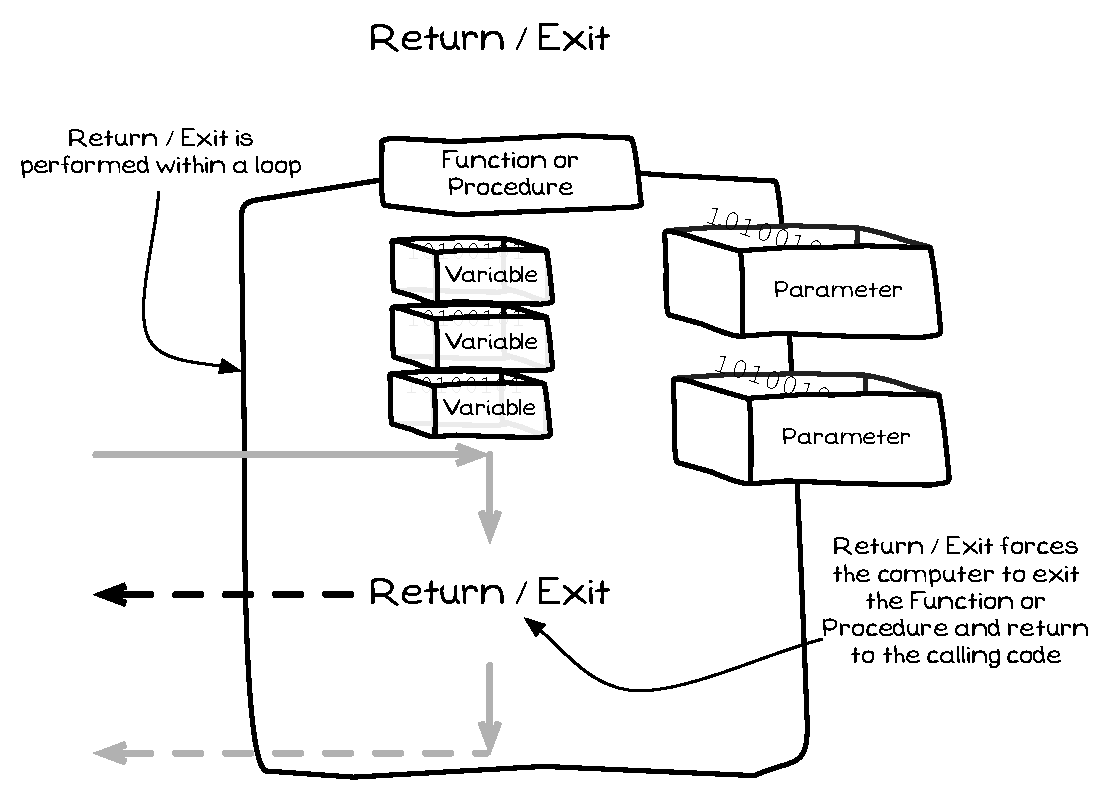
\includegraphics[width=\textwidth]{./topics/control-flow/diagrams/Return} 
   \caption{Exit ends the current Function or Procedure}
   \label{fig:exit}
\end{figure}

\mynote{
\begin{itemize}
  \item Exit is an \textbf{action}, allowing you to jump out of the current Function or Procedure, and return to the calling code.
  \item The Exit should be coded within a \nameref{sub:branching} statement that checks if the Function or Procedure should end.
\end{itemize}
}

\csection{C's version of the exit statement is the \nameref{sub:return_statement}. The return statement also provides the value that will be returned when exiting from a Function. As this sets the value to be returned you must have a return statement as the last action within a Function.}

% subsection return_or_exit_statement (end)
\clearpage
\subsubsection{Goto} % (fold)
\label{sub:goto}

The last jump statement is the goto statement. This is an unstructured jump, allowing you to jump anywhere in the code. Structured Programming principles called for the abolition of the goto statement. This is a statement you need to be aware of, but not one that should be used.

\begin{figure}[h]
   \centering
   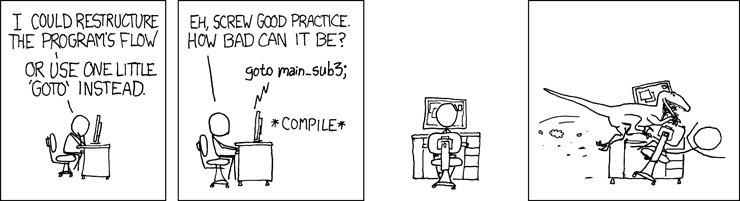
\includegraphics[width=\textwidth]{./topics/control-flow/images/goto} 
   \caption{The dangers of using goto, from \url{http://xkcd.com/292/}}
   \label{fig:goto}
\end{figure}

\mynote{
\begin{itemize}
  \item Goto is an action that allows you to jump to another instruction and continue from there.
  \item You need to be aware of the goto statement, but you should not use it.
\end{itemize}
}

% subsection goto (end)


\clearpage
\subsection{Compound Statement} % (fold)
\label{sub:compound_statement}

\nameref{sub:branching} and \nameref{sub:looping} statements need to be able to include a number of instructions within their paths. Often languages will manage this by indicating that only a \emph{single} statement can be included in any of these paths, and then include the ability to code multiple statements in a \emph{single compound statement}.

\begin{figure}[h]
   \centering
   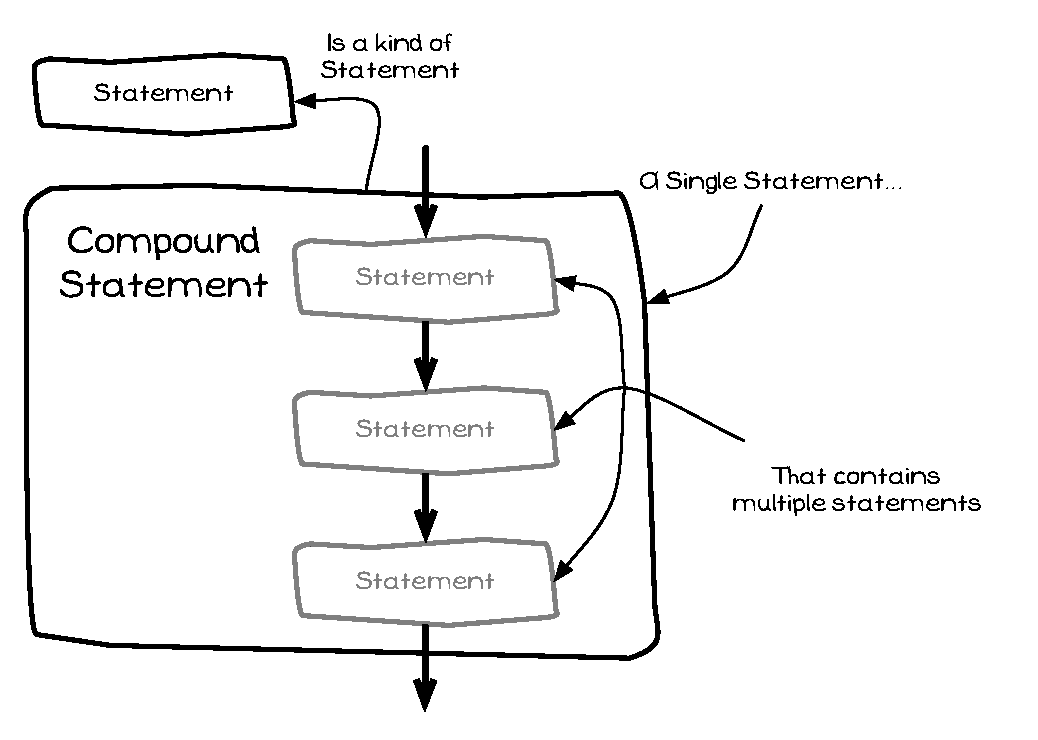
\includegraphics[width=\textwidth]{./topics/control-flow/diagrams/CompoundStatement} 
   \caption{A Compound Statement is a Statement that can contain other Statements}
   \label{fig:branching-compound-statement}
\end{figure}

\mynote{
\begin{itemize}
  \item A Compound Statement is a way of grouping \textbf{action}s, allowing you to create a single statement that contains multiple statements.
  \item Compound Statements are useful when combined with \nameref{sub:branching} and \nameref{sub:looping} Statements. Allowing you to put multiple statements within a path.
\end{itemize}
}

% subsection compound_statements (end)
\clearpage
\subsection{Statement (Simple and Structured)} % (fold)
\label{sub:statement_with_loops_}

Statements are the actions that we can get the computer to perform.  

\begin{figure}[h]
   \centering
   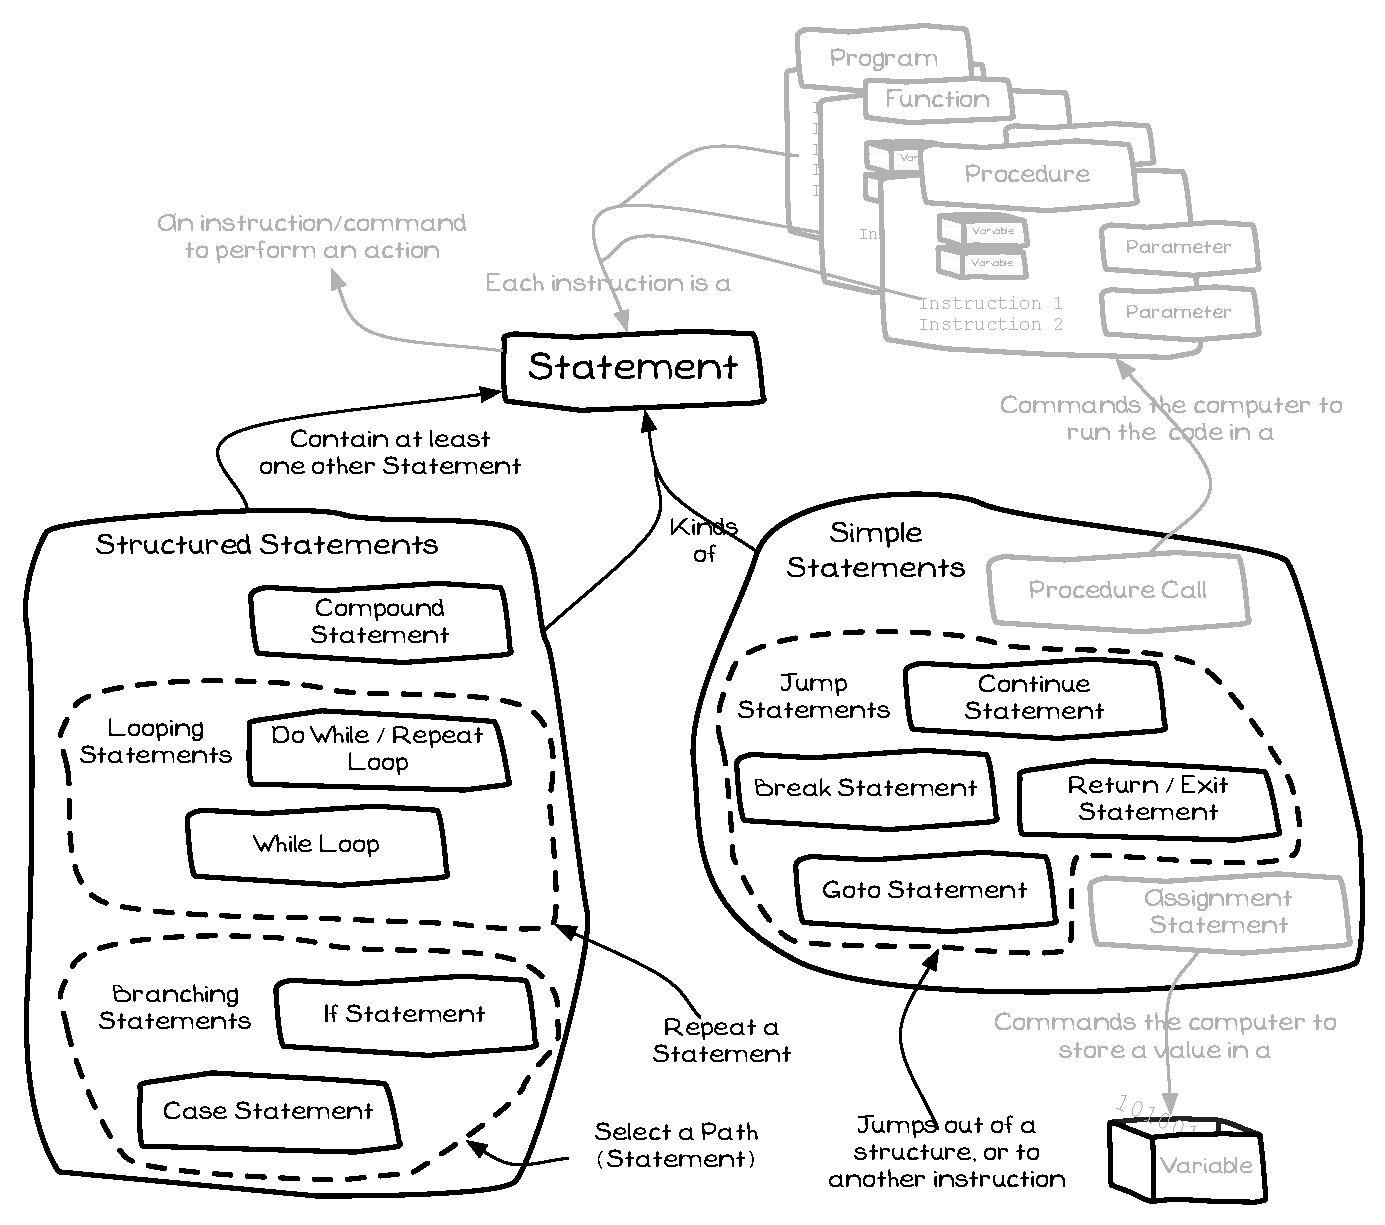
\includegraphics[width=0.88\textwidth]{./topics/control-flow/diagrams/Statement}
   \caption{A Statement may also be a Looping or Jumping Statement}
   \label{fig:looping-statement}
\end{figure}

\mynote{
\begin{itemize}
  \item Statement is the \textbf{term} given to the instructions in code.
  \item \textbf{Simple Statements} that perform an action. The actions you can perform are:
  \begin{itemize}
    \item \nameref{sub:procedure call} used to run the code in a Procedure.
    \item \nameref{sub:assignment_statement} used to calculate a value and store it in a Variable.
    \item Jump Statements allow you to affect which instruction will be performed next. This includes:
    \begin{itemize}
      \item \nameref{sub:break}: to jump out of a \nameref{sub:looping} Statement.
      \item \nameref{sub:continue}: jumps to the condition in a Looping Statement.
      \item \nameref{sub:exit}: (return in C) to end the current Function or Procedure.
      \item \nameref{sub:goto}: the unstructured jump\footnote{Often resulting in death by Raptor.} to an arbitrary location in the code.
    \end{itemize}
  \end{itemize}
  \item \textbf{Structured Statements} contain statements and control the flow of execution:
  \begin{itemize}
    \item \nameref{sub:looping} Statements: that repeat a statement a number of times.
    \begin{itemize}
      \item \nameref{sub:pre_test_loop}: Test condition before the body, repeating \textbf{0 to many} times.
      \item \nameref{sub:post_test_loop}: Test condition after the body, repeating \textbf{1 to many} times.
    \end{itemize}
    \item \nameref{sub:branching} Statement: that select from a number of optional statements.
    \begin{itemize}
      \item \nameref{sub:if_statement}: Branch based on a \nameref{sub:boolean_data} Expression (2 paths).
      \item \nameref{sub:case_statement}: Branch based on an Ordinal Expression (\emph{n} paths).
    \end{itemize}
  \end{itemize}
\end{itemize}
}


% subsection statement_with_loops_ (end)

\clearpage
\subsection{Summary} % (fold)
\label{sub:control_flow_summary}

This section has introduced a number of new actions that you can use in your code to create more dynamic programs. 

\begin{figure}[h]
   \centering
   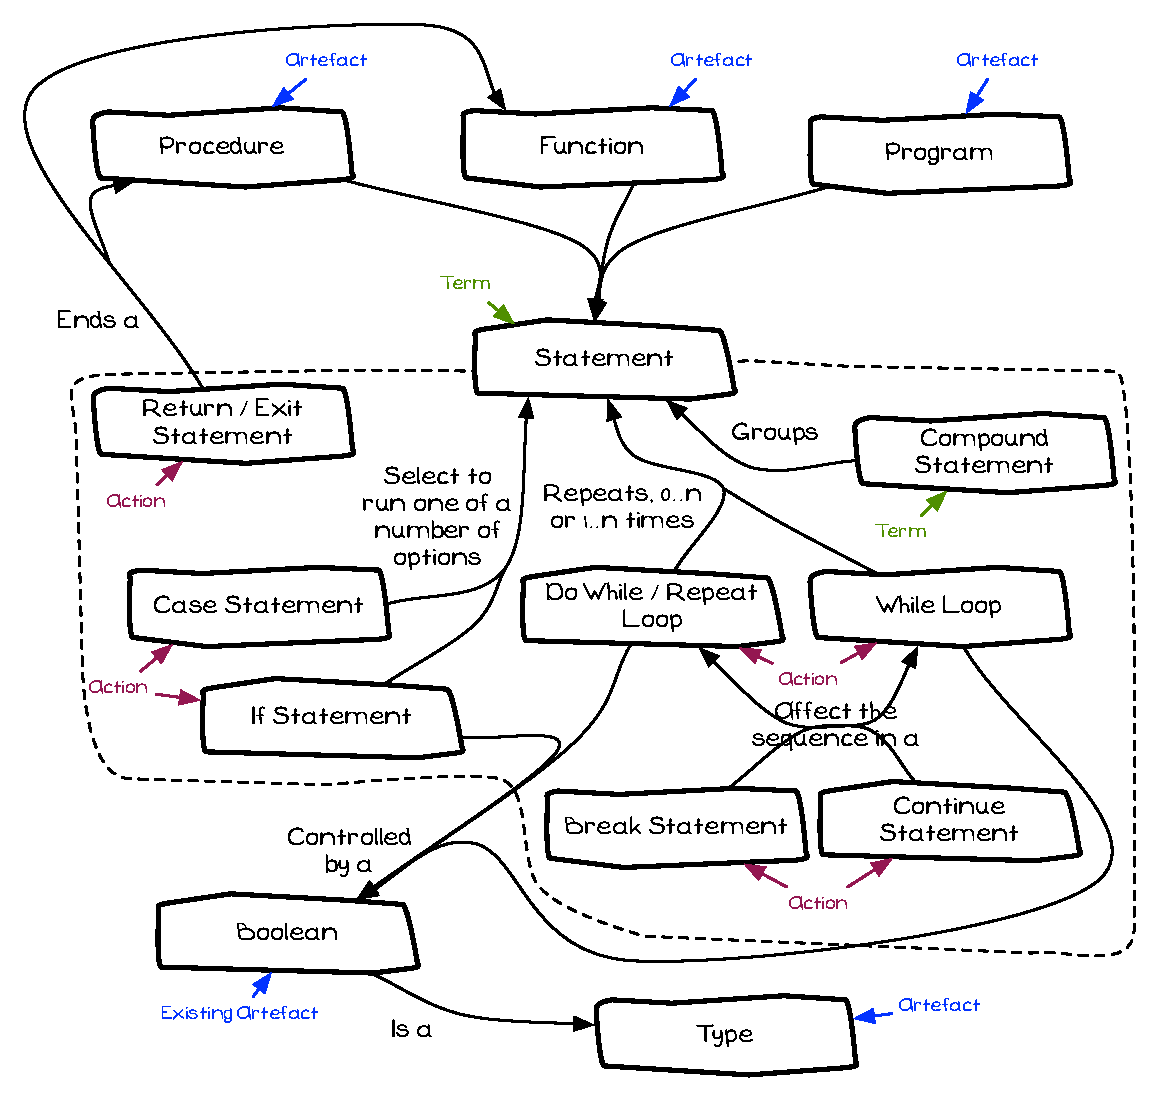
\includegraphics[width=\textwidth]{./topics/control-flow/diagrams/Summary} 
   \caption[Chapter Concepts]{Key Concepts introduced in this Chapter}
   \label{fig:control-flow-summary}
\end{figure}

\mynote{
\begin{itemize}
  \item \textbf{Artefacts} are things you can \emph{create} and \emph{use}.
  \item \textbf{Terms} are things you need to \emph{understand}.
  \item \textbf{Actions} are things you can \emph{command} the computer to perform.
\end{itemize}
}

% subsection summary (end)
% section control-flow_concepts (end)
